%%%%%%%%%%%%%%%%%%%%%%%%%%%%%%%%%%%%%%%%%%%%%%%%%%%%%%%%%%%%
\section{Gas system} \label{sec:GasSystem}

The functions of the gas system of NEXT-DEMO are the evacuation of the detector, its pressurization and depressurization with xenon (and argon), and the recirculation of the gas through purification filters. A schematic of the system is shown in figure~\ref{fig:GasSystem}.

%%%%%%%%%%
\begin{figure}[tbh]
\centering
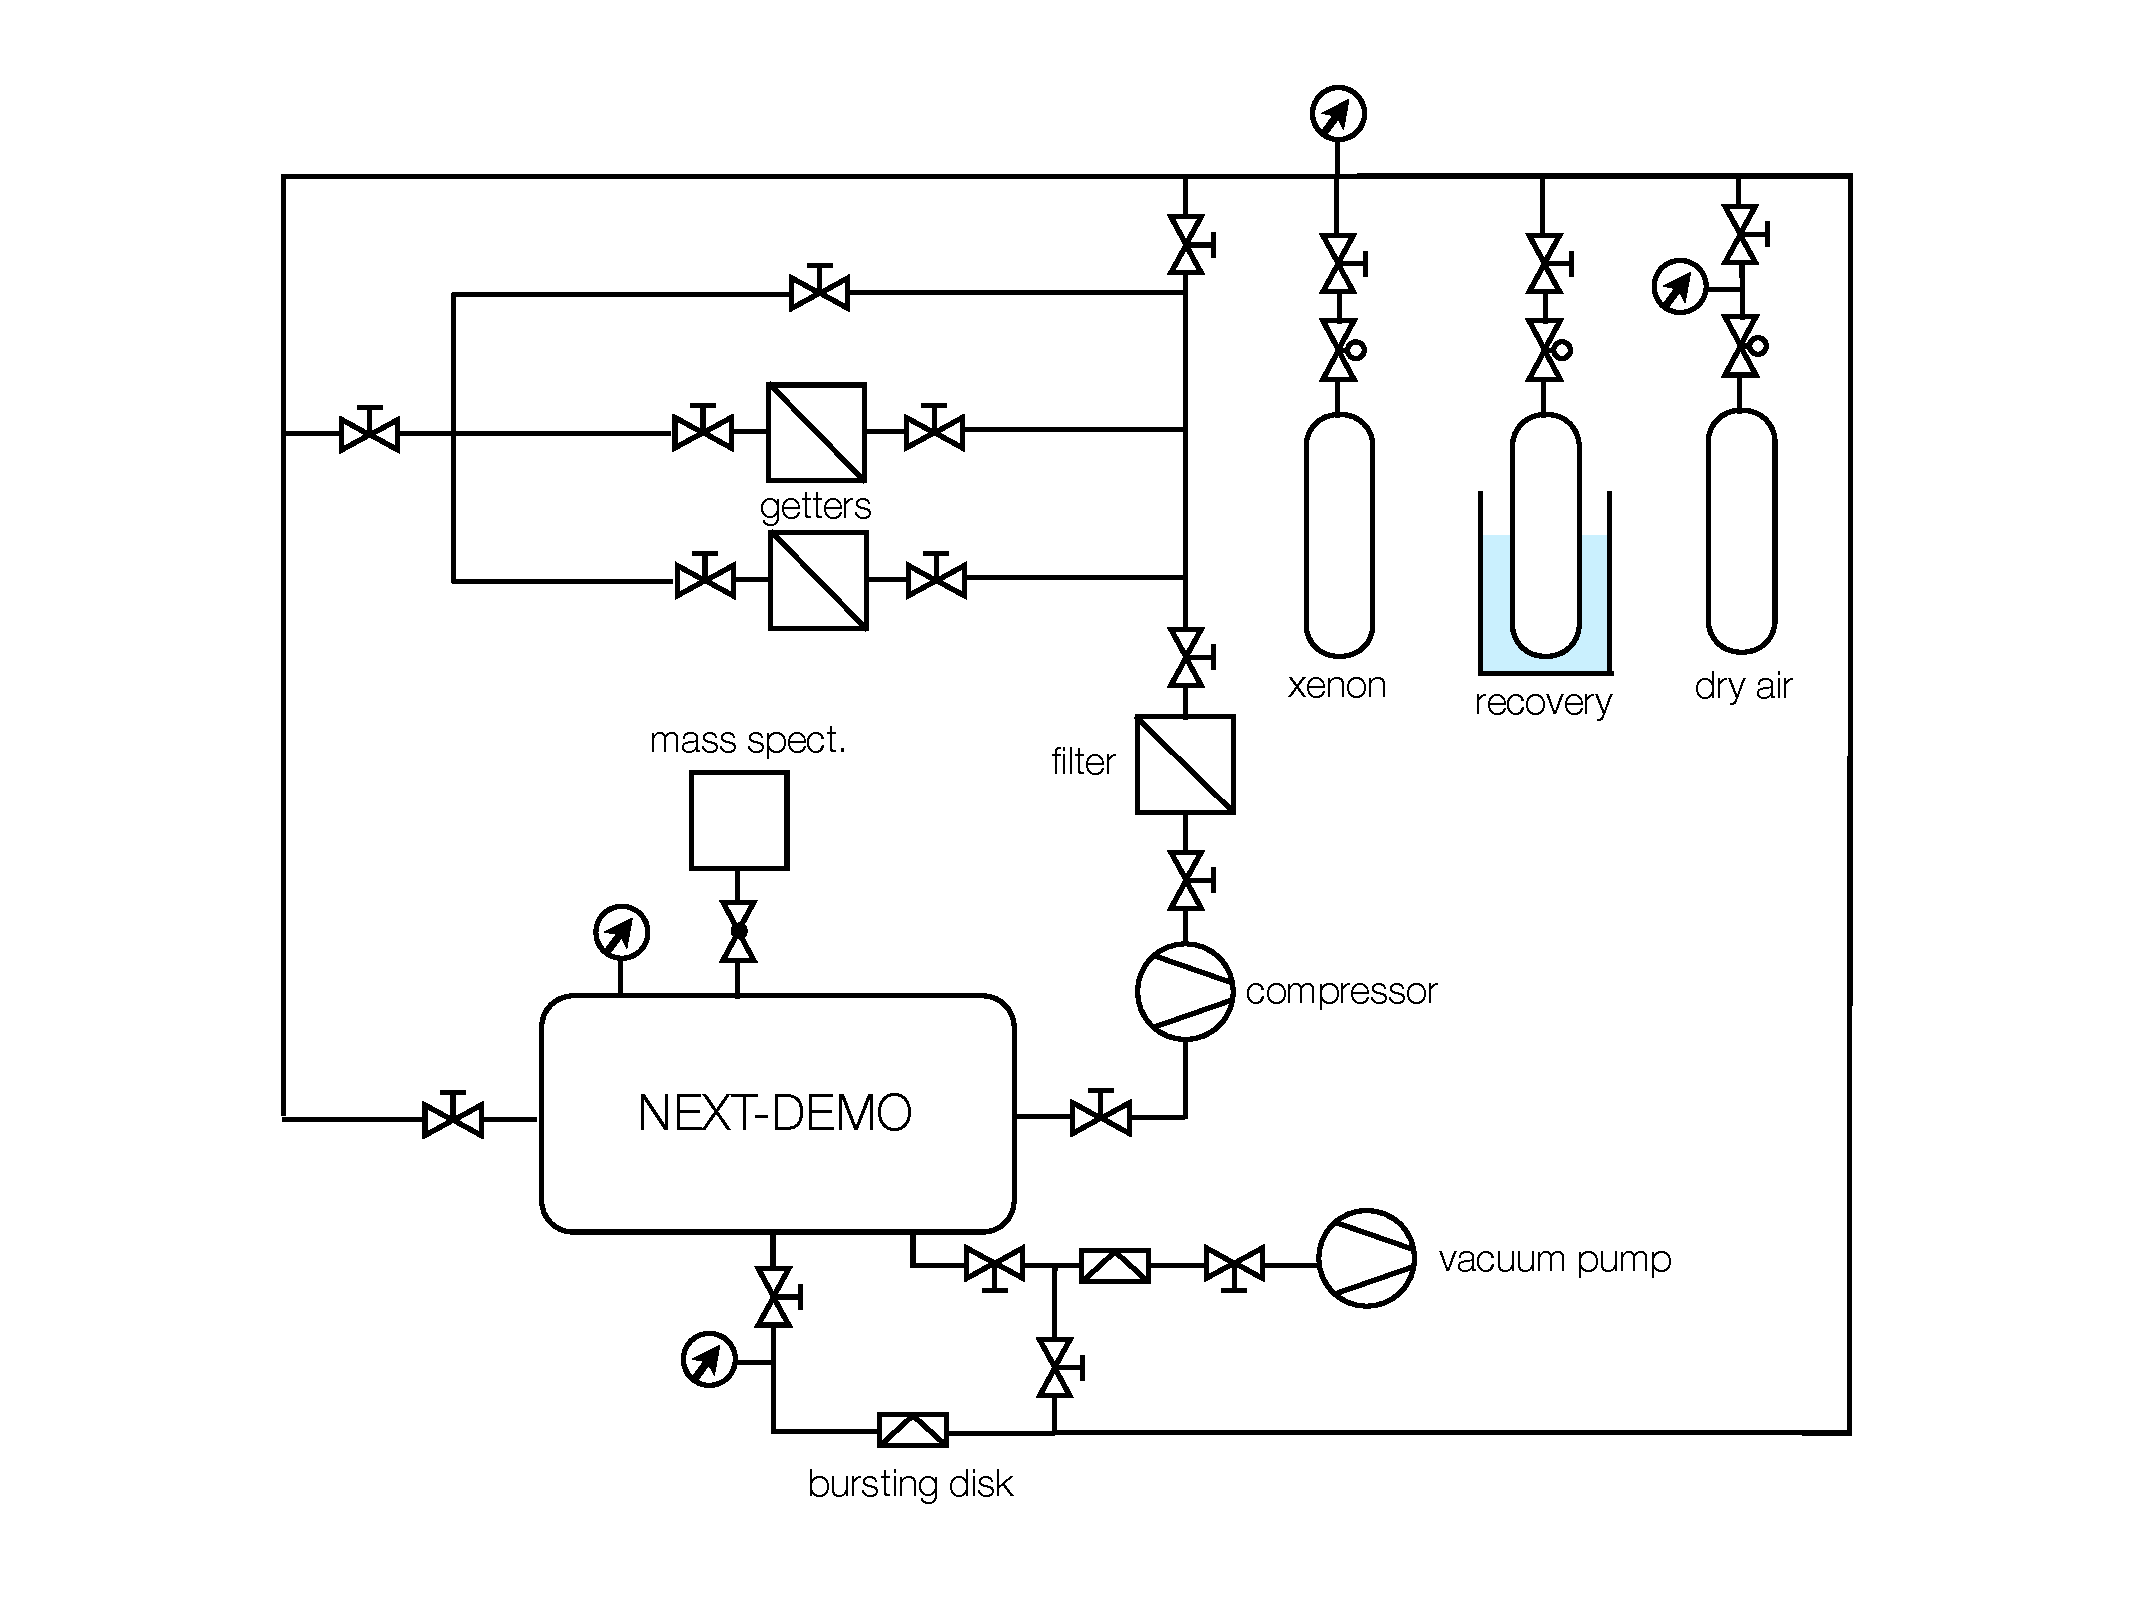
\includegraphics[width=\textwidth]{img/GasSystem.pdf}
\caption{Simplified schematic of the gas system of NEXT-DEMO.} \label{fig:GasSystem}
\end{figure}
%%%%%%%%%%

The standard procedure during normal operation of the detector starts with the evacuation of the vessel to vacuum levels around $10^{-5}$~mbar. The detector is then filled with xenon gas to pressures up to 10 bar. The xenon can be cryogenically recovered to a stainless-steel bottle (Fig. \ref{fig:RecoB}) connected to the gas system by simply immersing this in a dewar filled with liquid nitrogen. The gas flows inside the bottles and freezes there.
%The pressure regulator of the bottle is fully opened to allow the xenon gas to flow inside it (due to the temperature difference) and freeze.

%%%%%%%%%%
\begin{figure}[tbh]
\centering
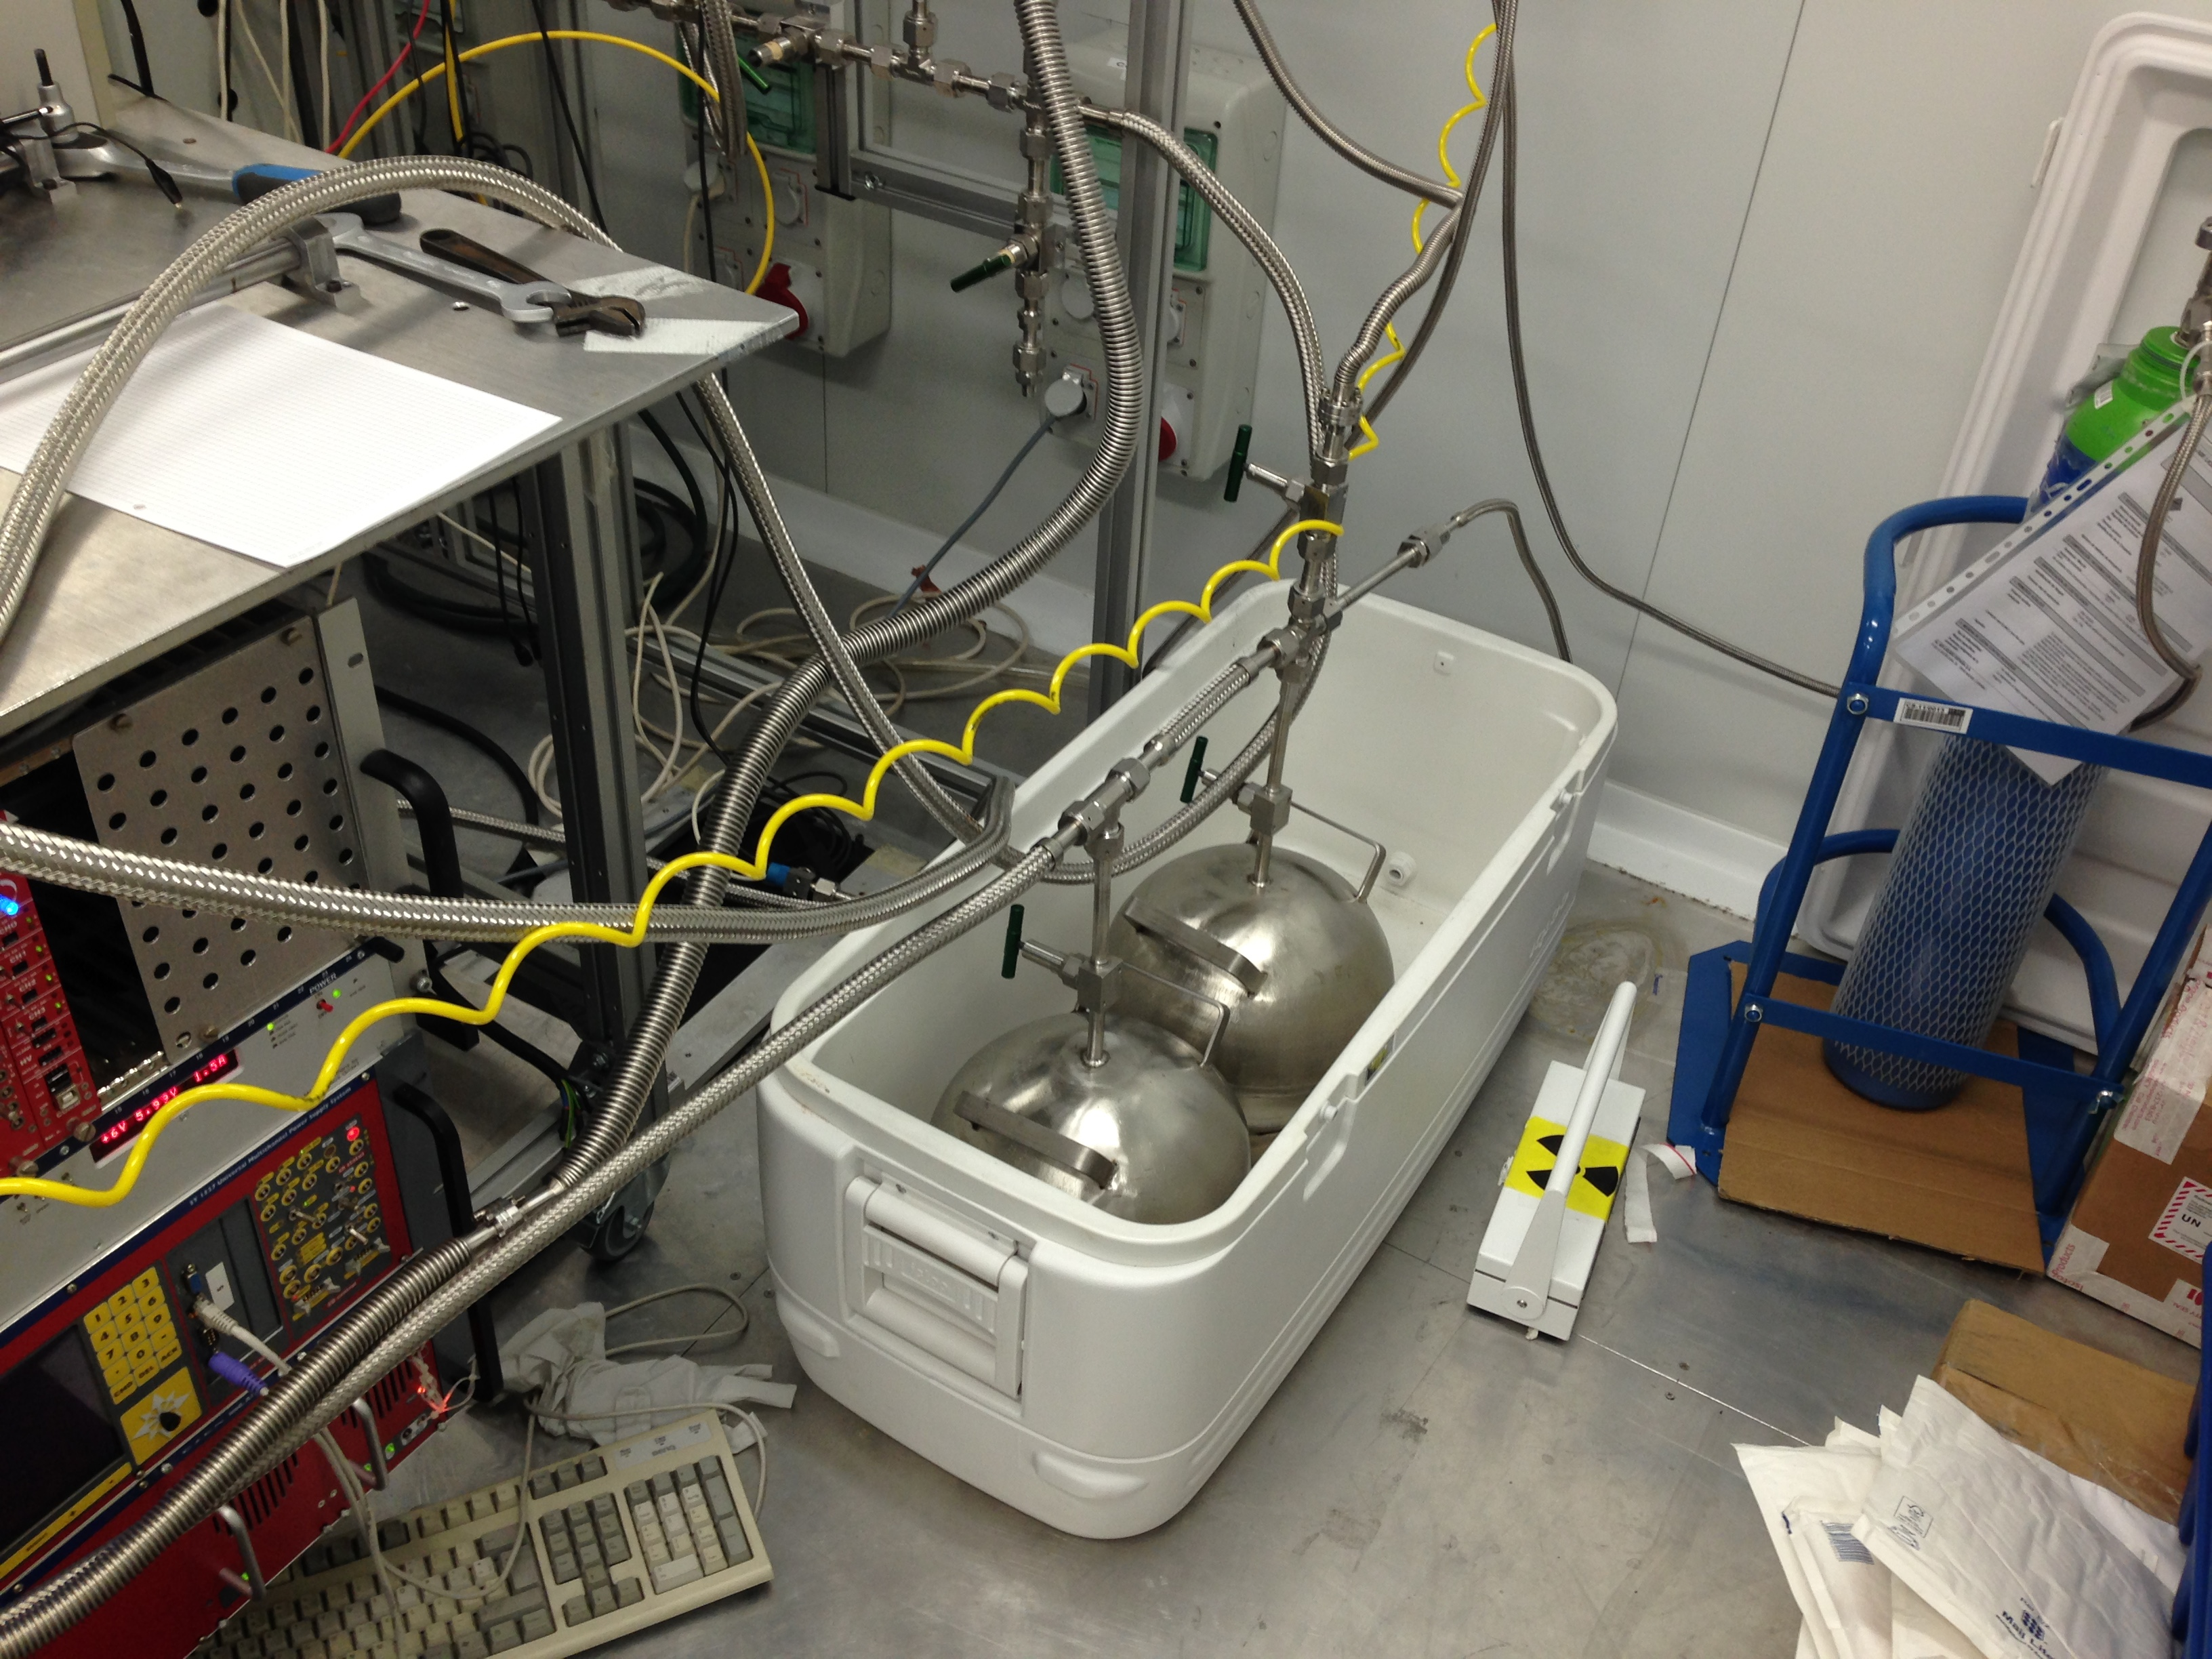
\includegraphics[width=\textwidth]{img/recoverybottle.jpg}
\caption{Stainless steel bottles used for cryogenic recovery of the Xenon} \label{fig:RecoB}
\end{figure}
%%%%%%%%%%



The vacuum pumping system consists of a roughing pump (Edwards XDS5 scroll vacuum pump) and a turbo molecular pump (Pfeiffer HiPace 300). Vacuum pressures better than $10^{-7}$~mbar have been obtained after pumping out the detector for several days. The recirculation loop is powered by an oil-less, single-diaphragm compressor (KNF PJ24999-2400) with a nominal flow of 100 standard liters per minute. This translates to 
an approximate flow of 10 liters per minute at 10 bar, thus recirculating the full volume of NEXT-DEMO ($\sim45$~L) in about 5 minutes. The gas system is equipped with both room-temperature (SAES MC50) and heated \emph{getters} (SAES PS4-MT15) that remove electronegative impurities (O$_{2}$, H$_{2}$O, etc.) from the xenon. All the gas piping, save for the inlet gas hoses and getter fittings, are $1/2$ inch diameter with VCR fittings. A set of pressure relief valves (with different settings for the various parts of the system) and a burst disk in the vacuum system protect the equipment and personnel from overpressure hazards.

The operation of the gas system (Fig. \ref{fig:GasSystem2}) has been, in general, very stable. The detector has run without interruption for long periods with no leaks and continuous purification of the gas. However, one major leak occurred when the diaphragm of the recirculation pump broke, causing the loss of the xenon volume contained in the chamber. This led to the installation of an emergency mechanism that, in the event of pressure drop, automatically closes those valves connecting the pump to the rest of the gas system. Since installation, only one major failure has taken place which the emergency system isolated without loss of gas.  Micro-leaks, on the level of 0.005 bar per day, due to bad connections in the gas system have also been detected making it necessary to introduce additional xenon to maintain pressure. The micro-leaks where found and properly repaired allowing for a stable detector operation in the last year.

%%%%%%%%%%
\begin{figure}[tbh]
\centering
\includegraphics[width=\textwidth]{img/GasSystem2.jpg}
\caption{Picture of the Gas system used in the NEXT-DEMO detector.} \label{fig:GasSystem2}
\end{figure}
%%%%%%%%%%


Several improvements to the initial design of the gas system have been made thanks to the initial data runs. These include the recognition of the importance of reliability of the main pump as well as the decision to use hot getters as the main gas purification stage due to their negligible emission of radon compared to that of room-temperature getters.

\subsection{Cryo-recovery protocol}

When the gas system needs to be stopped for an intervention in the detector the gas Xenon needs to be recovered and saved. The way of recovering the Xenon from the vessel and the gas system is with cryogenics.

NEXT-DEMO gas system has two spherical bottles specially designed for this use (see attachements) that are connected to the vessel and to the gas system. The bottles are placed in a thermally insolated container that is filled with liquid nitrogen until it reaches (approx.) half of the height of the bottles. Once the nitrogen stops boiling we open the corresponding valve to the part of the system that we want to recover, vessel or gas system. It is also possible to have both open at the same time if needed. Then the Xenon flows into the recovery bottles where it frezzes.

Once the pressure in the vessel/gas system is stable at ~0.03 absolute bar the bottles are full and we close them. Then we need to wait for the liquid nitrogen to evaporate.



\subsection{Gas Mixtures}

For the updgrade of NEXT-DEMO++ we will need to operate the detector with a mixture of Xenon with other gas. The gas choosen as a first option is CO$_2$. This gas give us all the advantages of the gas mixtures (improvement in drift velocity, reduction of diffusion,...) at concentrations smaller than 1\% . In order to control the concentration of CO$_2$ the gas system will need a small upgrade consisting in two flow meters and a small bottle of CO$_2$.


\subsection{Technical and safety specifications}

The gas system is made up of standard components. The Getters and the compressor carry CE marks.

Swagelock components do not carry a CE mark. However, all Swagelock
components used comply with the requirement of Article~3, Paragraph~3 of the PED Directive \mbox{(97/23/EC)} and in accordance with that section do not carry a CE mark. Notwithstanding, we can included all the certificates.

The complete list of parts with the associated part numbers is given in attachment "VALCI-MONTI-195". We have also selected a list of major components that is given below, in which we have omitted explicit listing of the standard components such as elbows and similar coupling as they are too numerous and being all manufactured by Swagelock comply with the above mentioned PED directive.


%bellow. We have omitted explicit listing of the standard components such as elbows and similar coupling as they are too numerous and being all manufactured by Swagelock comply with the above mentioned PED directive.
%
\begin{itemize}

\item  28 $\times$ 1/2Ó VCR valves SS/8BG-VCR
\item  3 $\times$ 1/4Ó VCR valves 6LVV-DPHVR4-P1
\item  2 $\times$ 1/4Ó VCR valves SS-4BC-VCR
\item  3 $\times$ regulators KPR1JRFX27A20000

\item  2 $\times$  Cold getters SAES Pure Gas MC450-902
\item  1 $\times$  Hot getter SASE Pure Gas PS4-MT15-R2

\item  Compressor: 1 $\times$ KNF PJ24999-2400
\end{itemize}


Non standard components are:
The Vessel and the Stainless steel recovery bottles which were specifically designed and tested for NEXT. The calculations and test document are included in the attachment document to this one.




%\subsection{Technical and safety specifications}
%
%The gas system has been built and assembled by Swagelock. All the different parts have the safety certificate for pressure operation in the attached documents.

